% !TEX root =  ../master.tex
\chapter{Nutzerhandbuch} %TODO: Das hier eventuell nochmal überarbeiten und kürzen?
Bei der Endwicklung der Anwendung haben wir großen Wert auf eine intuitive Gestaltung der \ac{GUI} und der \ac{UX} gelegt.
% TODO: ist das eine nicht-funktionale Anforderung?
Ziel war es, eine Anwendung zu gestalten, deren Nutzer die Anwendung ohne Erklärung verstehen.
Dennoch möchten wir in diesem Kapitel ein Referenzhandbuch erstellen.
In diesem Kapitel wird beschrieben, wie Nutzer die Anwendung verwenden können.

% TODO: Bilder müssen überall rein
\section{Öffnen der Anwendung}
Die Anwendung kann jederzeit \href{https://dhbwlearning.web.app}{\enquote{dhbwlearning.web.app}} geöffnet werden.
Wie jede andere Webapplikation kann dies über jedes Gerät, welches über eine Internetverbindung verfügt durch einen Webbrowser geöffnet werden.
Das heißt, die Anwendung steht den 24\,h pro Tag bereit und kann von allen Studenten und Dozenten verwendet werden.

\section{Login}
Nach dem Öffnen der Anwendung wird der Nutzer in der Regel aufgefordert sich einzuloggen.
In \autoref{fig:login} ist die Anmeldeseite dargestellt.

\begin{figure}[h]
    \centering
    \includegraphics[width=.7\textwidth]{img/Login.png}
    \caption{Login-Maske}
    \label{fig:login}
\end{figure}

Für die Anmeldung muss der Nutzer die Email-Adresse zu seinem Account, sowie das entsprechende Passwort angeben.
Setzt der Nutzer einen Hacken bei \enquote{Remember me}, so wird der Nutzer beim nächsten starten der Anwendung nicht um ein Password gebeten und wird automatisch in seinen Account eingeloggt.

Sollte der Nutzer noch keinen Account haben kann er auf \enquote{Register} klick, um sich selbst für die Nutzung der Anwendung zu registrieren.
Genaueres zur Registrierung sind in \autoref{sec:registrierung} beschrieben.

Sollte der Nutzer bereits einen Account haben und nur das Password zu diesem vergessen haben gibt es neben dem Password-Feld einen \enquote{Forgot Password?}-Button.
Dieser leitet den Nutzer zu einem Password-Vergessen-Formular weiter, welches in \autoref{sec:passwordVergessen} beschrieben ist.

Hat der Nutzer eine korrekte Email- und Passwordkombination eingetragen und auf \enquote{Login} geklickt, wird der Nutzer auf das Dashboard (vgl. \autoref{sec:dashboard}) weitergeleitet.
Andernfalls wird der Nutzer freundlich darauf hingewiesen, dass das Password nicht korrekt ist.



\section{Registrierung}\label{sec:registrierung}
Die Registrierungs-Maske dient dazu, einen neuen Nutzer in der Anwendung anzulegen.
Damit sich Nutzer registrieren können müssen sie eine Email-Adresse sowie ein Password wählen.
Der Nutzer kann hierbei eine beliebige, sogar eine Wegwerf-Email verwenden.
Die Email wird intern lediglich für Authentifizierungszwecke benötigt.
Das heißt die Email wird nur für das Login und für den Fall, dass ein Nutzer sein Passwort vergessen hat benötigt (vgl \autoref{sec:passwordVergessen}).
Verwendet der Nutzer eine Wegwerf-Email kann der die Anwendung wie gewohnt nutzen, verliert aber die Möglichkeit sein Passwort zurückzusetzen.

Das Password kann frei gewählt werden, solange es mindestens 6 und maximal 50 Zeichen hat.
Es gibt keine weiteren Einschränkungen, da wir der Meinung sind, dass aufwändige Passwortvorgaben eine schlechte \ac{UX} ergibt.
Dennoch sollten Nutzer Passwörter verwenden, die allgemein als sicher gelten.
% TODO: Vielleicht nochmal sagen, das wir sicher sind, weil firebase google auth?
Um zu verhindern, dass sich der Nutzer bei seinem Passwort vertippt hat, muss das Passwort ein zweites Mal bestätigt werden.

Schließlich muss der User den Nutzungsbedingungen zustimmen.
% TODO:

Sollte der Nutzer bereits einen Useraccount besitzen kann er jederzeit durch einen klick auf \enquote{Log in} zur Login-Maske zurückkehren.

Ist alles korrekt ausgefüllt kann der Nutzer durch klick auf \enquote{Registrieren} die Anmeldung abschließen und wird automatisch eingeloggt.

Direkt nach der Registrierung wird der Nutzer auf eine Seite mit verschiedenen Fragen weitergeleitet. Diese Seite beinhaltet Fragen zu seinem Lerntypen. 
Der Nutzer kann die Fragen freiwillig beantworten, jedoch helfen sie dem Dozenten einen Überblick zu bekommen, welche verschiedenen Lerntypen in 
einem Kurs enthalten sind. Die Auswertung der Lerntypen wird unter dem Punkt \autoref{sec:Feedback} weiter behandelt.

\begin{figure}[h]
    \centering
    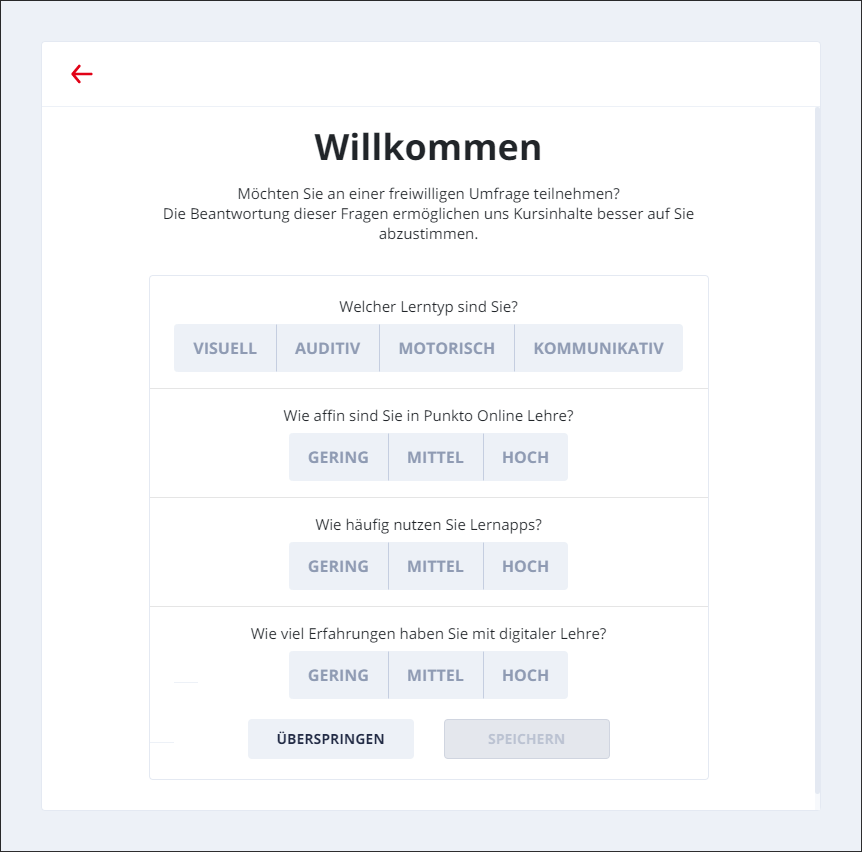
\includegraphics[width=.7\textwidth]{img/Einstiegsfragen.png}
    \caption{Einstiegsfragen}
    \label{fig:einstiegsfragen}
\end{figure}


\section{Password-Vergessen}\label{sec:passwordVergessen}
Die Password-Vergessen-Funktion dient zum Zurücksetzen des Passwortes.
Möchte der Nutzer sein Password zurücksetzen und erneut Zugang zu seinem Account bekommen kann der Nutzer jederzeit seine Email in das Password-Vergessen-Feld eingeben.

\begin{figure}[h]
    \centering
    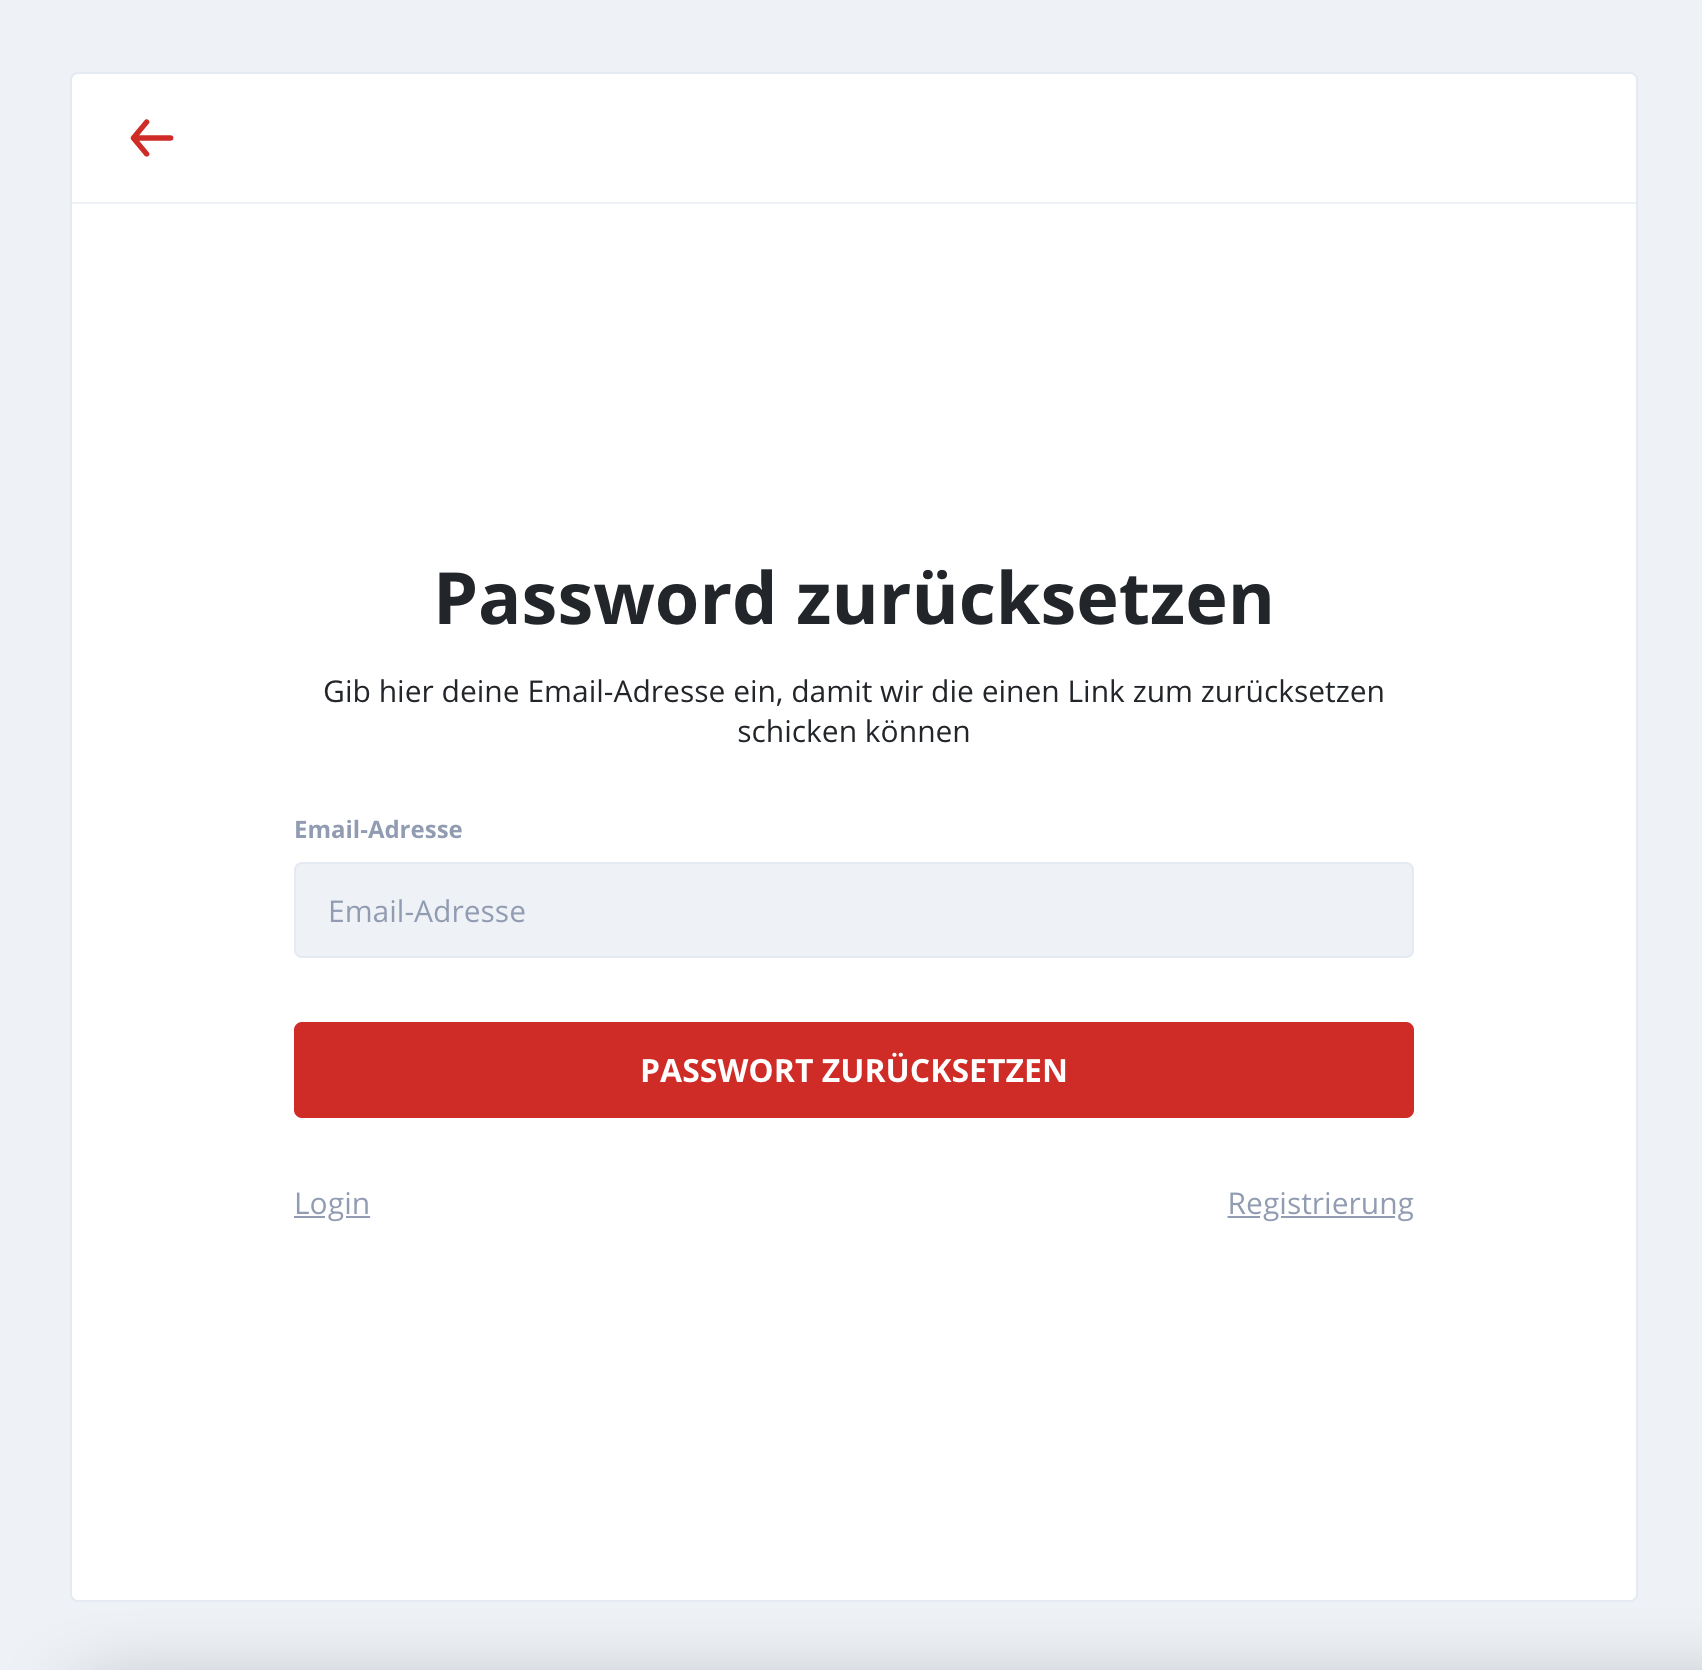
\includegraphics[width=.7\textwidth]{img/Passwort_zuruecksetzen.png}
    \caption{Password-Vergessen-Maske}
    \label{fig:passwordVergessen}
\end{figure}

Nachdem der Nutzer auf \enquote{Request Password} geklickt hat wird automatisch eine Email an die angegebene Email-Adresse gesendet.
Die Email enthält einen Link, mithilfe dem der Nutzer sein Passwort ändern kann.
Der Link leitet den Nutzer auf die in \autoref{fig:passwordVergessen} dargestellte Maske in der der Nutzer sein Passwort ändern kann.
Hat der Nutzer sein Passwort geändert wird der zu einem erneuten Login auf die Login-Maske geleitet.

Anzumerken ist, dass der Link zum Passwort ändern nur einmal gültig ist.
Sollte das Passwort bereits geändert worden sein, muss eine neue Email angefordert werden.
Dies verhindert, dass unberechtigte Personen die Email mitlesen können und das Passwort erneut ändern könn

% TODO: Muss man hier jede kleinigkeit schreiben? also das email auch wirklich eine email sein muss?


\begin{figure}[h]
    \centering
    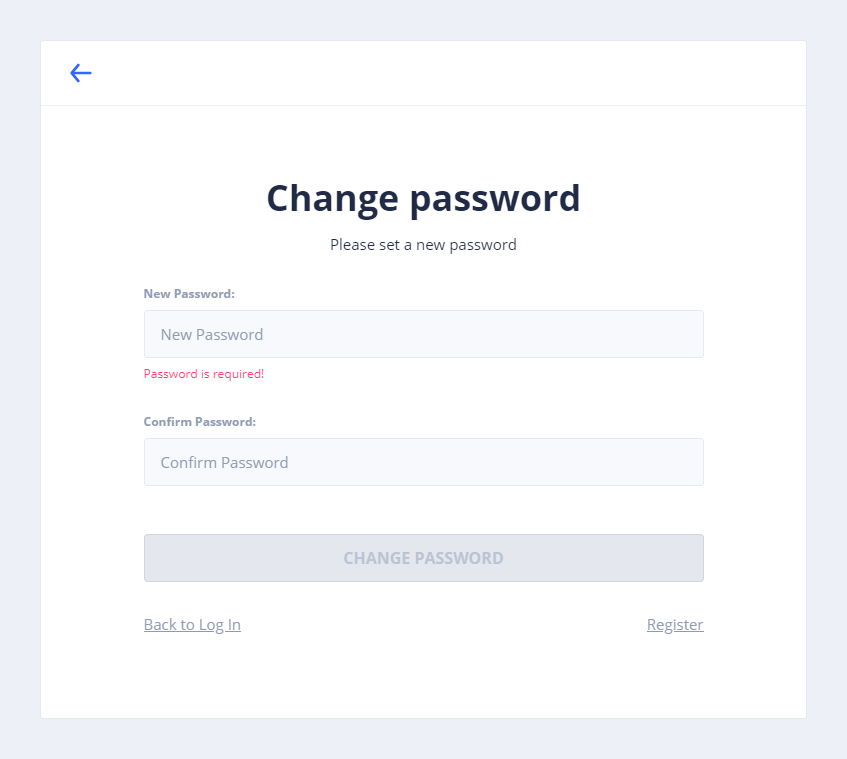
\includegraphics[width=.7\textwidth]{img/passwordReset2.png}
    \caption{Password-Aktualisieren-Maske}
    \label{fig:passwordVergessen2}
\end{figure}

% ..


\section{Dashboard}\label{sec:dashboard}
Das Dashboard ist die erste Seite, die der Nutzer sieht, wenn er sich erfolgreich eingelogt hat. Es soll einen Überblick über alle bevorstehenden Ereignisse geben.
Die nächsten anstehenden Prüfungen werden in einem Kalender angezeigt und Gesamtanzahl an Prüfungen wird auch eingeblendet. In der Übersicht können nochmal die wichtigsten 
Informationen zu der Prüfung eingesehen werden, wie zum Beispiel die Uhrzeit und der Raum. 
\begin{figure}[h]
    \centering
    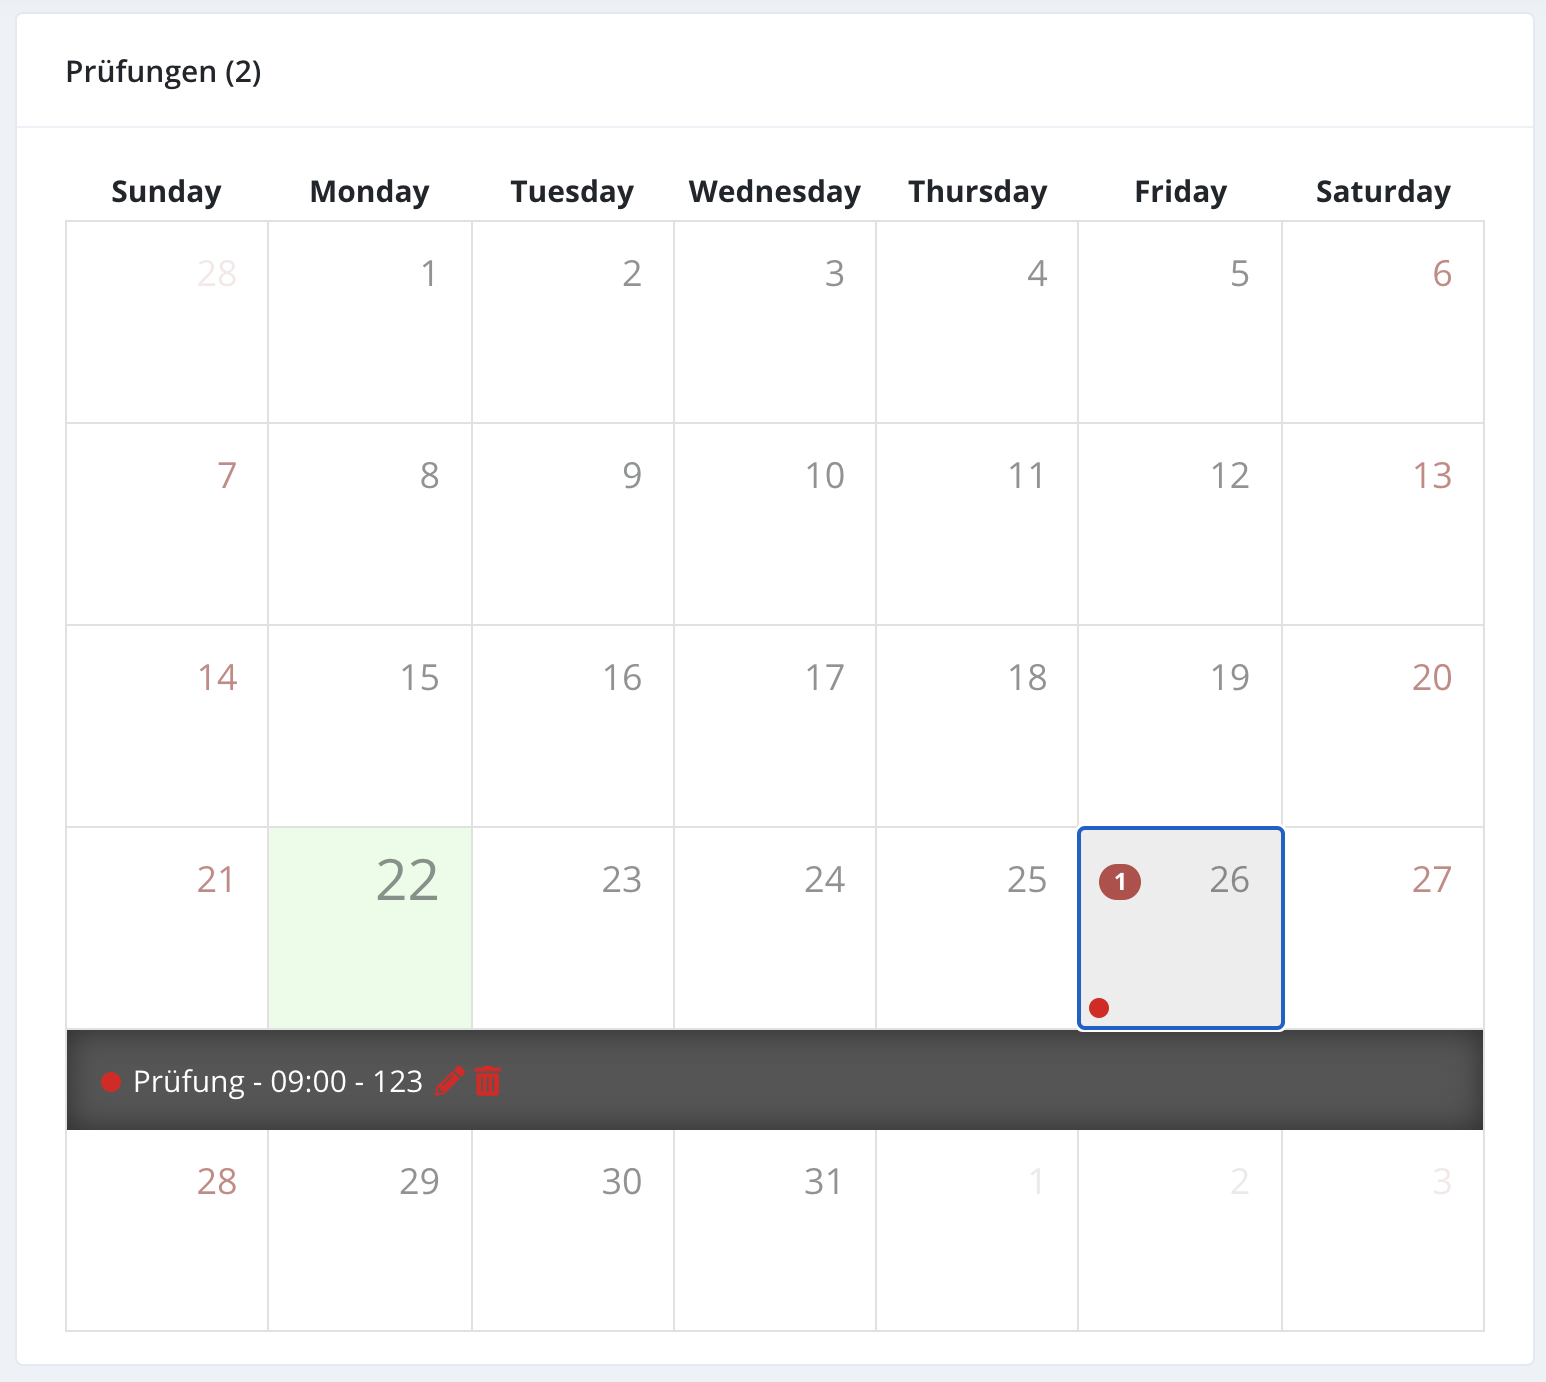
\includegraphics[width=.7\textwidth]{img/Dashboard_3.png}
    \caption{Dashboard-Prüfung}
    \label{fig:Dashboardansicht}
\end{figure}
Zusätzlich zu den nächsten Prüfungen werden auch bald fällige Aufgaben angezeigt. Der Benutzer sieht auf einen Blick, wie viele Tage er noch für welche Aufgabe hat.
\begin{figure}[h]
    \centering
    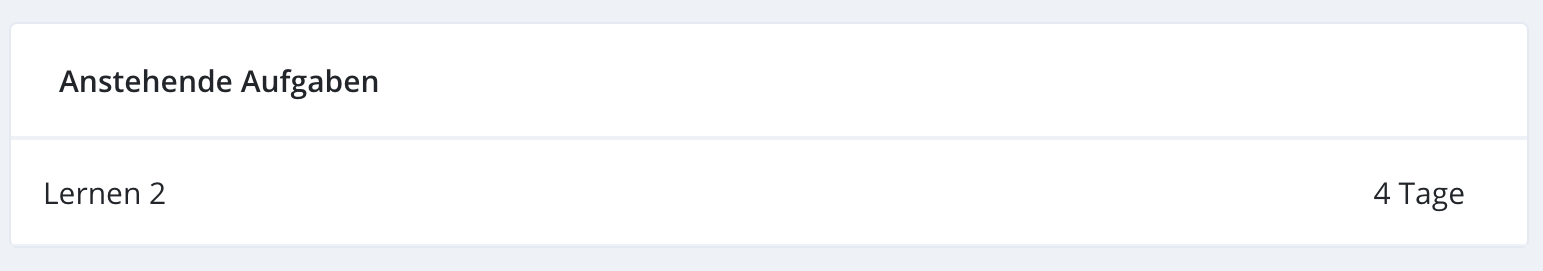
\includegraphics[width=.7\textwidth]{img/Dashboard_4.png}
    \caption{Dashboard-Aufgaben}
    \label{fig:Dashboardaufgaben}
\end{figure}

\section{Karteikarten}\label{sec:Karteikarten} % TODO: Bilder
Index-Cards stellen eine Karteikarten-Funktion dar. Dabei können Dozenten neue Karteikarten erstellen, die die Kursteilnehmer bearbeiten können.
Im Nutzer-Interface werden diese Karten ähnlich zu einem realen Karteikasten hintereinander dargestellt.
Jede Karte zeigt zunächst die Frage an.
Solle man die Antwort zu der Frage nicht wissen oder sich kontrollieren wollen, kann man mithilfe des Pfeils im Eck einer jeden Karte die Antwort einblenden.
Anschließend können die Karten mit den Buttons am unteren Bildschirmrand als gewusst und nicht gewusst markiert werden.
Durch die Zahlen an diesen Buttons kann der Nutzer leicht ablesen, wie viele Karten der Nutzer bereits wusste.
Karten können aber auch durch einfaches ziehen der Karten zu gewusst oder nicht gewusst verschoben werden.
Dies erleichtert die Handhabung. In der Abbildung \autoref{fig:Karteikarten} ist die Ansicht zu sehen, die ein Teilnehmer bekommt, wenn er die Karteikarten durcharbeitet.
\begin{figure}[h]
    \centering
    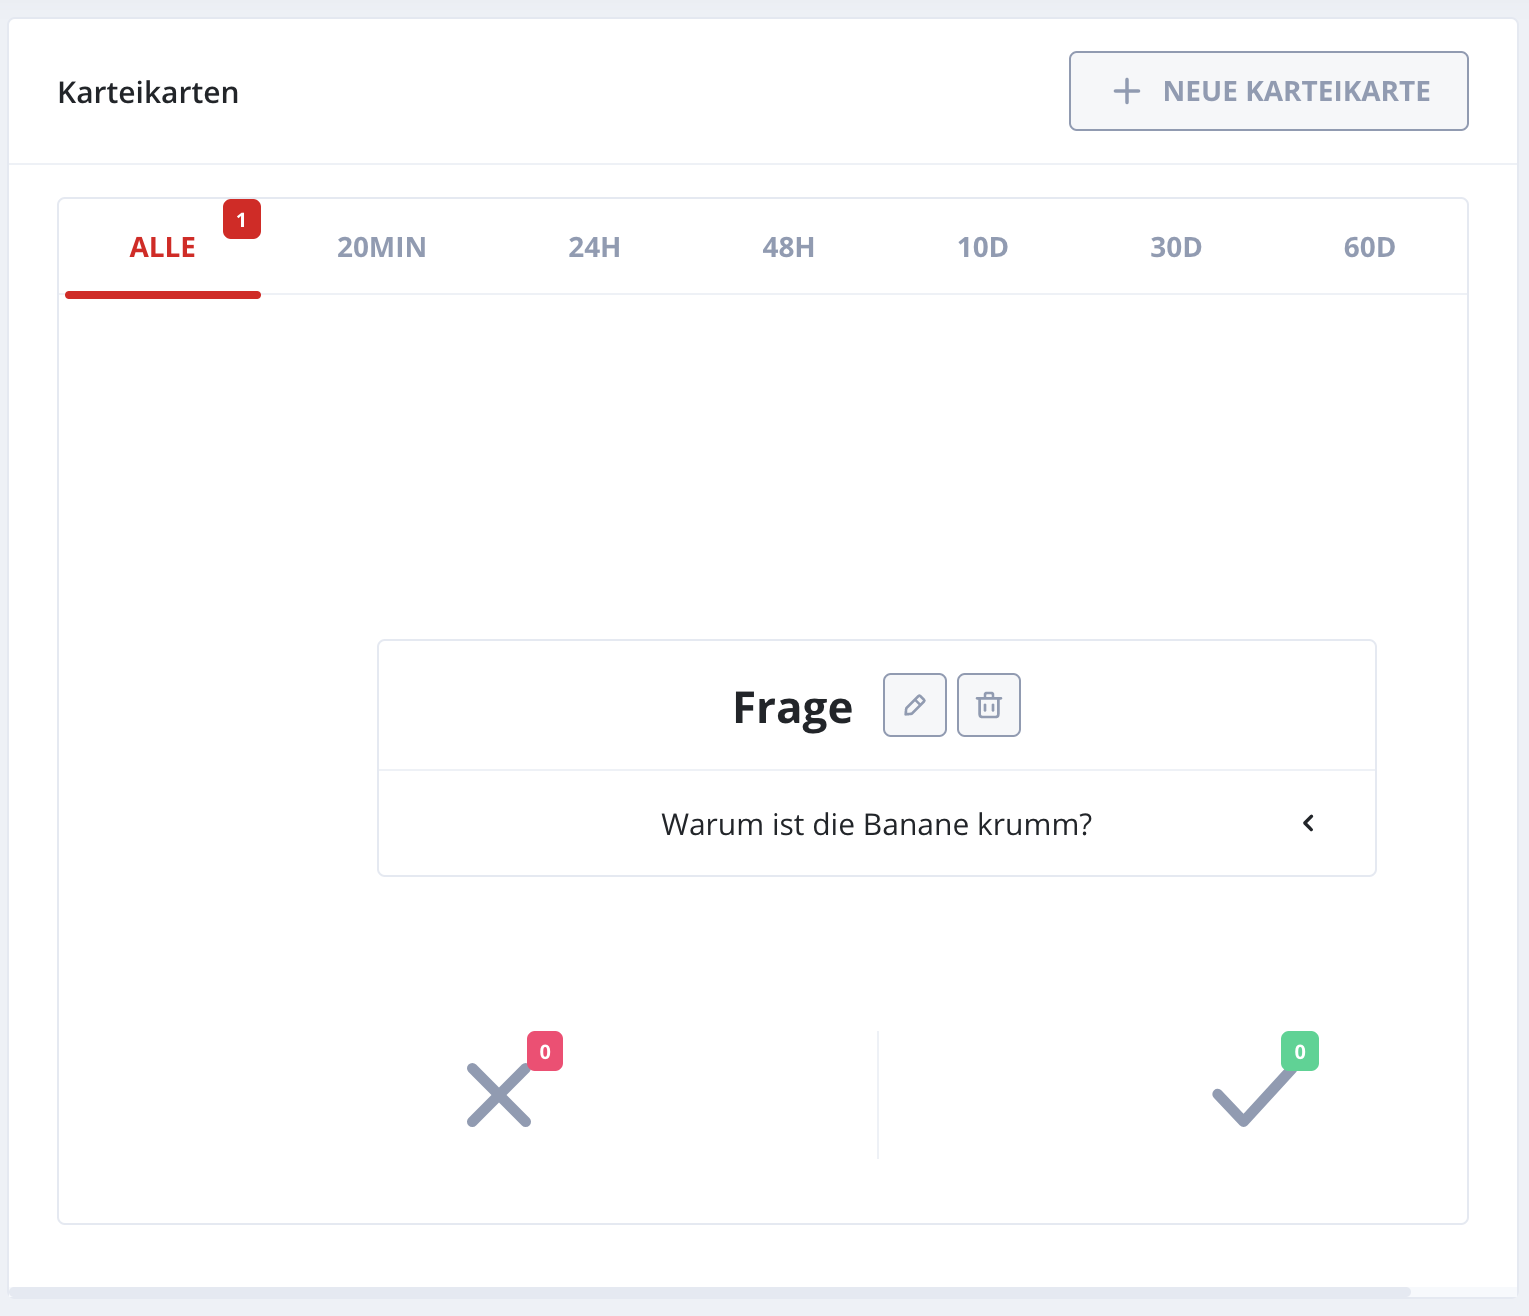
\includegraphics[width=.7\textwidth]{img/Karteikarten_hinzugefuegt.png}
    \caption{Karteikarten}
    \label{fig:Karteikarten}
\end{figure}

Wurden alle Karteikarten beantwortet bekommt der Student direkt Feedback, wieviel Prozent aller Fragen er richtig beantworten konnte.
% TODO: Zusätzlich bekommt er angezeigt, welche Karten er nocheinmal auffrischen sollte
% TODO: Erstellung


\section{Aufgaben}\label{sec:Aufgaben} % TODO:
Aufgaben stellen einen elementaren Bestandteil einer Ausbildung dar.
Schon in der Schule mussten Schüler eine Hausaufgabenheft oder Ähnliches führen um einen Überblick über ihre Aufgaben zu haben.
Auch im Studium gibt es Unzähliche Aufgaben, wie zum Beispiel das Erstellen von Zusammenfassungen.

Aufgaben können mithilfe des \enquote{Floating Action Button (FAB)} im rechten unterem Eck erstellt werden. % https://material.io/components/buttons-floating-action-button#usage
Fabs stellen die primäre Action einer Ansicht, die konstruktiv ist und zu dem Inhalt der Ansicht passt.
Inner


% TODO: Die Material Principien besser herausarbeiten  https://material.io/components/dialogs#usage
Nach dem Klick öffnet sich ein Modal, in dem alle relevanten Aufgaben eingetragen werden können.
Aufgaben zeichnen sich durch einen Titel und eine optionale Beschreibung, sowie eine optionale Deadline aus.
Sofern eine Deadline angegeben ist, wird dieses Aufgabe in dem Kalender über der Aufgaben Übersicht dargestellt.
Je roter ein Tag ist, desto mehr Aufgaben müssen an diesem Tag erledigt sein.
Der Kalender zeigt stets den Zeitraum zwischen Anfang des letzten Monates und Ende der nächsten zwei Monate  an.
% TODO: ?
Aufgaben können schnell und einfach durch klicken auf die Checkbox vor einer Aufgabe abgehackt werden.
In der Abbildung \autoref{fig:Aufgabeanlegen} ist bereits eine Aufgabe angelegt und es ist zu sehen in welchem Zeitraum diese Aufgabe erledigt werden muss.
\begin{figure}[h]
    \centering
    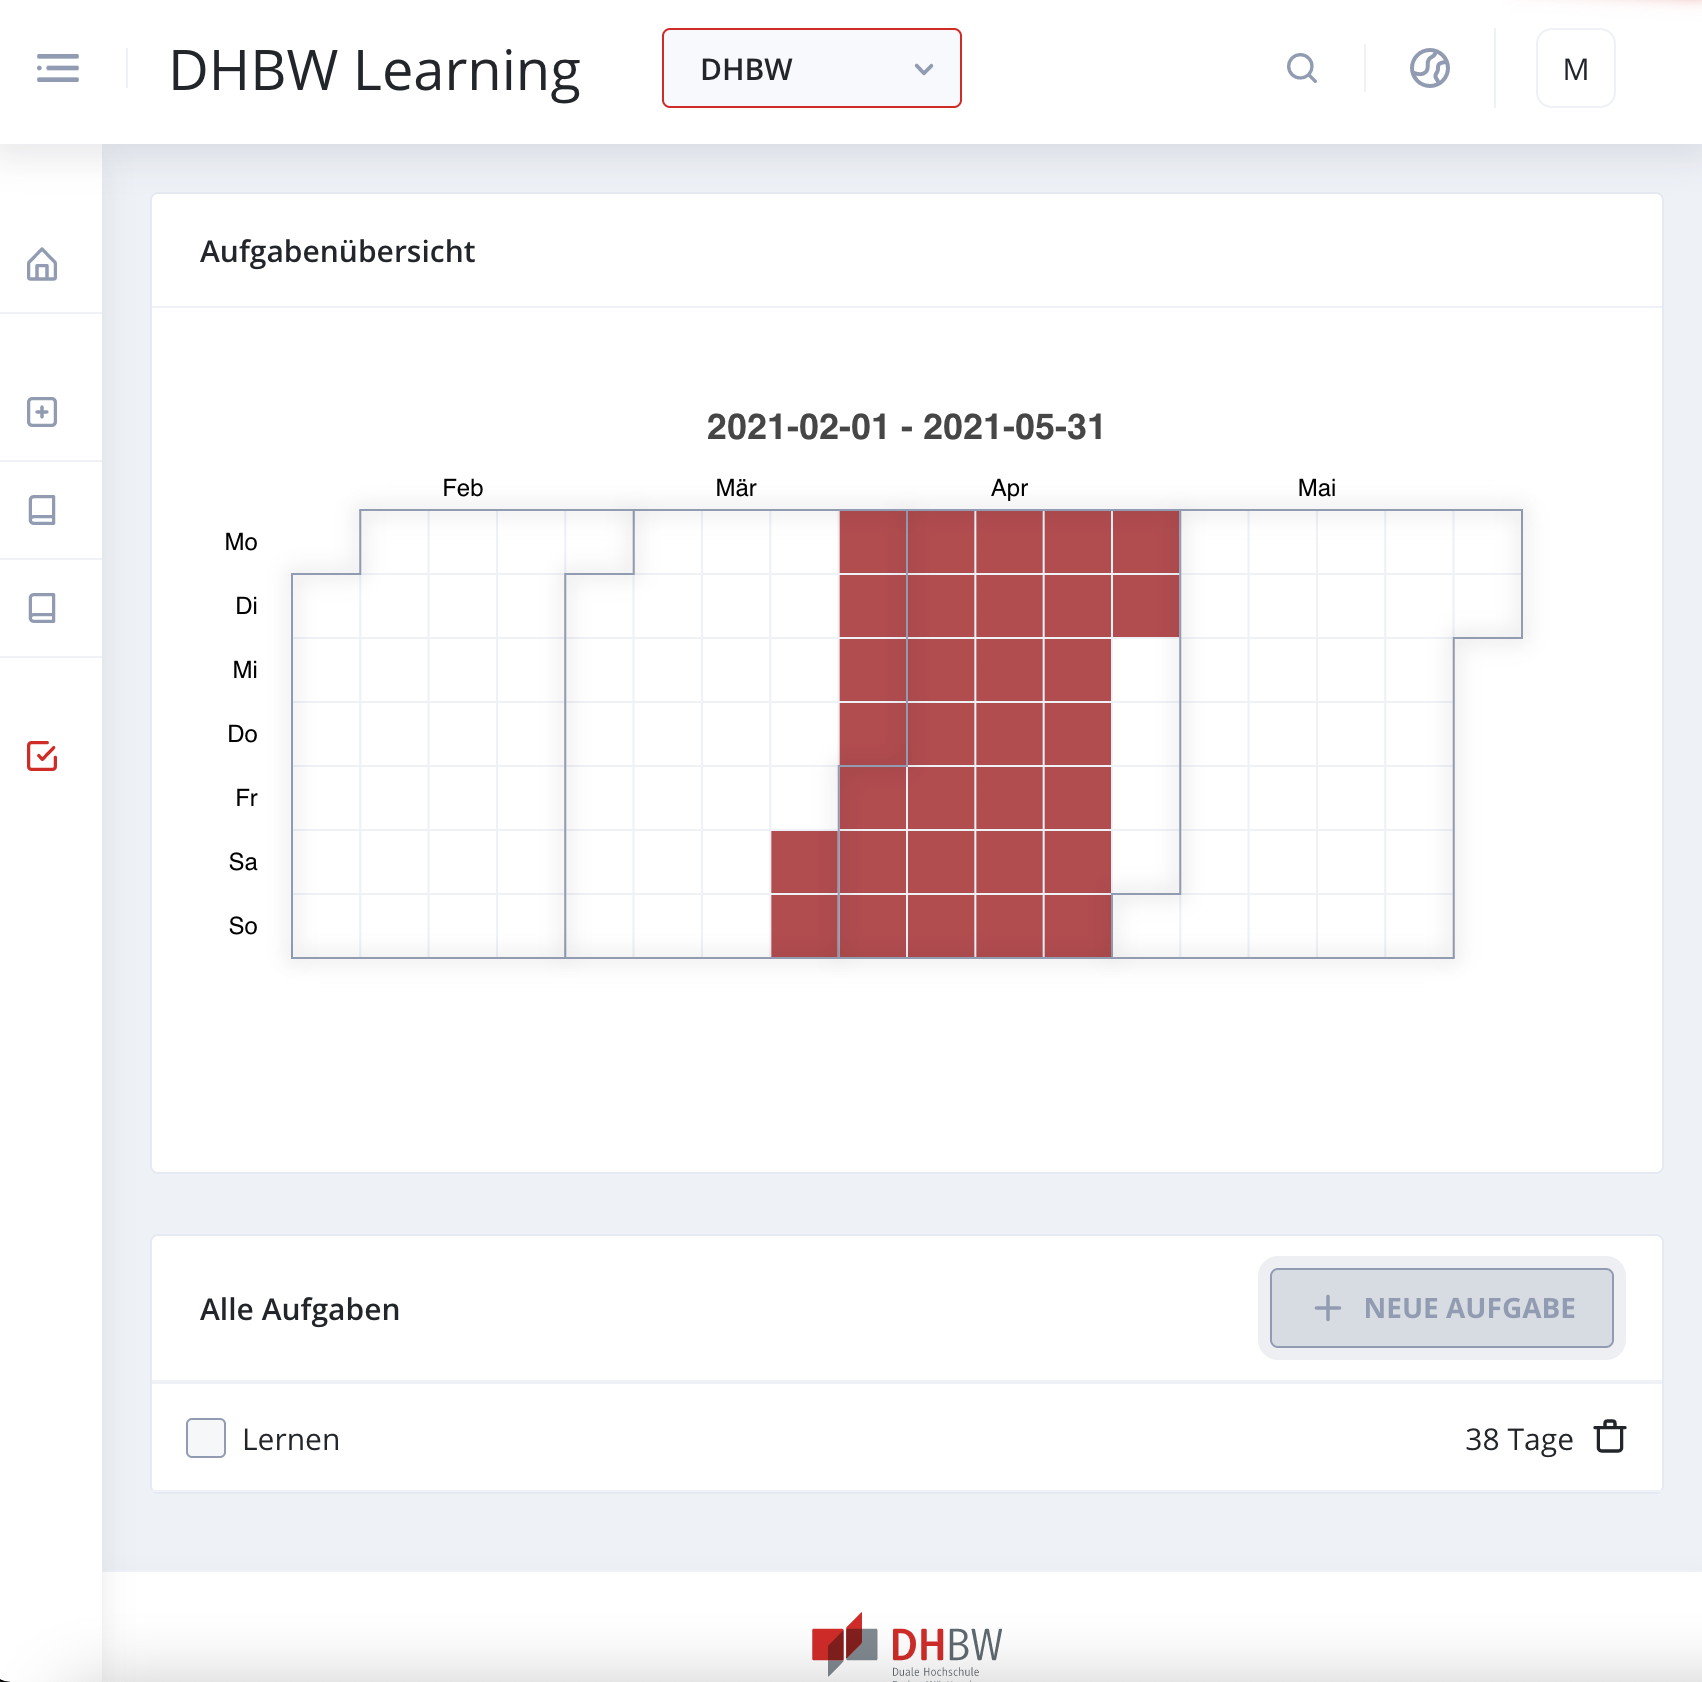
\includegraphics[width=.7\textwidth]{img/Aufgabe_angelegt.png}
    \caption{Aufgabe angelegt}
    \label{fig:Aufgabeanlegen}
\end{figure}




% TODO: Das hier schreiben, wenn da tatsächlich was implementiert ist

% TODO: Kurs einschreibung, ...



\section{Dateien}
Die \enquote{Dateien}-Maske dient zur Verwaltung von Dokumenten.
% TODO: Das in Konzeption verschieben?
Momentan müssen Dokumente umständich an Studenten weitergegeben werden.
In der Regel werden Dokumente an die Studiengangsleiter geschickt, welche die Dokumente anschließend weiterverteilen.
Das Problem ist, dass zuerst die Email-Adressen dieser ausgetauscht werden müssen und diese einen zusätzlichen Aufwand haben.
So sind neue oder korrigierte Dokumente nur schwer auszutauschen.
Auch Dokumente, die während einer Vorlesung verteilt werden müssen, erzeugen eine Zeitdifferenz.
Dazu kommt, das dieser Workflow nicht immer gleich ist.
Oft bekommen verschiedene Schülter unterschiedliche Informationen.
In einigen Fällen wird auch Moodle für die Dateiablage verwendet.

Aus diesem Grund wird ein einheitliches System benötigt, in dem Dateien abgelegt werden können.

\begin{figure}[h] 
    \centering
    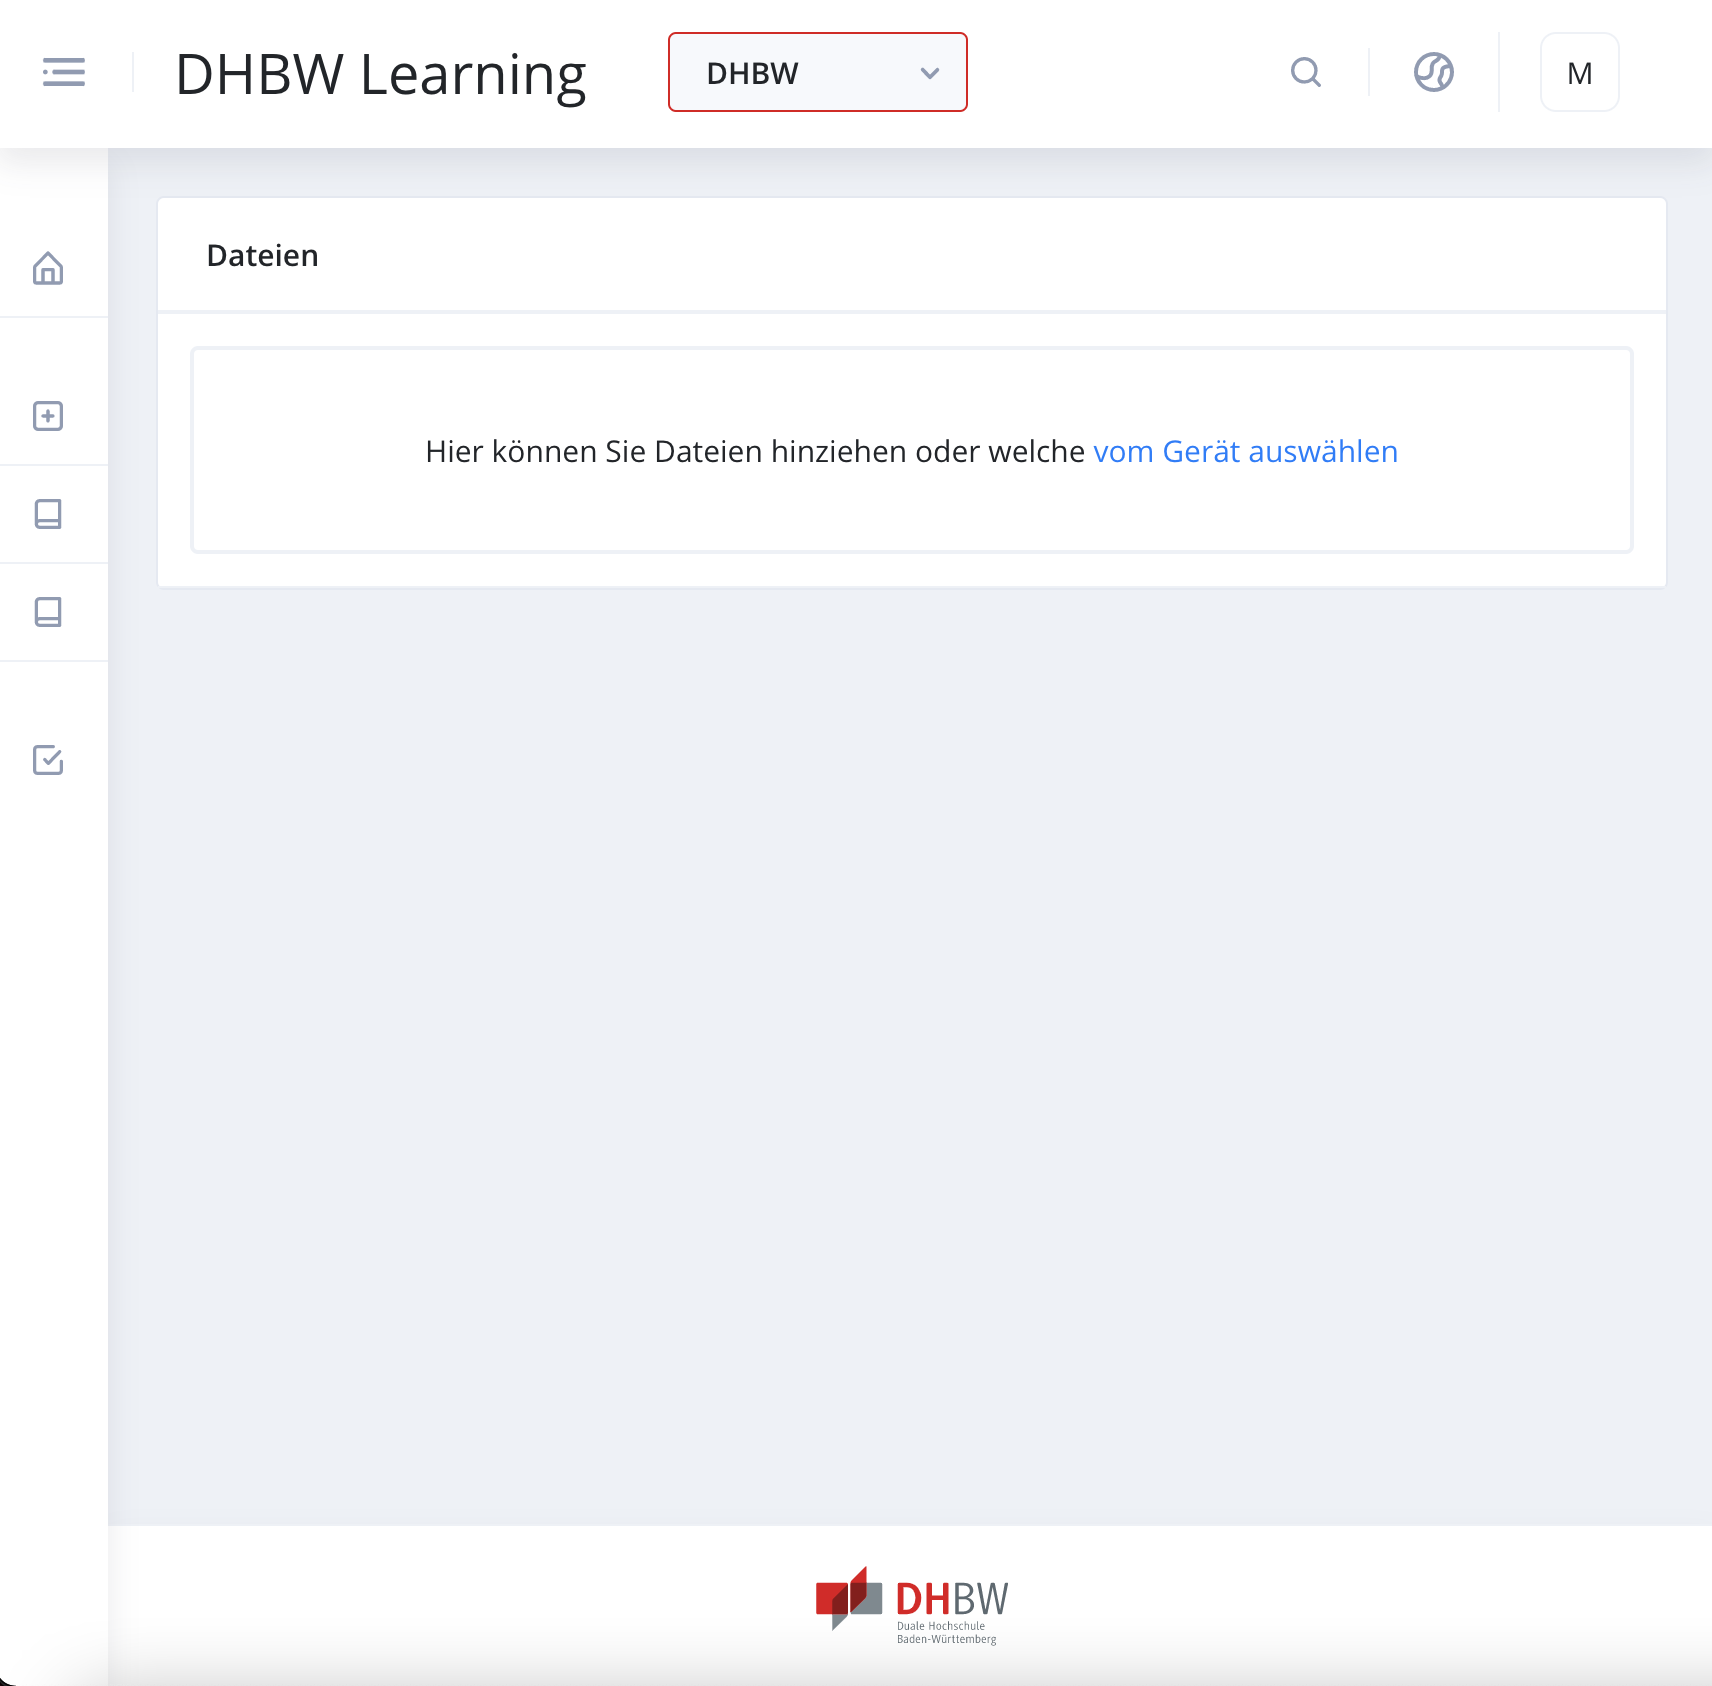
\includegraphics[width=.7\textwidth]{img/Dateien_uebersicht.png}
    \caption{Dateien-Maske}
    \label{fig:dateien}
\end{figure}

Das in \autoref{fig:dateien} dargestellte Datenmanagementsystem erleichtert dies, da Dokumente für einen Kurs hochgeladen werden können.
Dokumente können mithilfe des \enquote{browse}-Button hochgeladen werden.
Dafür öffnet sich ein Fenster, in dem beliebig viele Dateien für den Upload hochgeladen werden.
Zur einfacheren Nutzung können optional auch Dateien direkt aus dem Explorer in das Fenster gezogen werden.

Anschließend werden die Dateien hochgeladen.
Ein Fortschrittsbalken zeigt dabei stets den aktuellen Upload-Fortschritt an.
Anschließend können die Dokumente von allen Studenten heruntergeladen werden.
% TODO: Buttons rechts?

% TODO: Müssen die Toasts auch erklärt werden?

Bei der Nutzung des Dateisystems ist darauf zu achten, dass aus Speichergründen nicht alle Dateien antizipierend heruntergeladen werden können.
Dies würde es ermöglichen Geräte von Studenten zu überfordern.
Besonders Mobilgeräte besitzen noch einen begrenzten Speicher.
Aus diesem Grund muss während der Benutzung auf eine Internetverbindung geachtet werden.
Offline können nur die existierenden Dateien angezeigt werden, aber weder neue hochgeladen noch bestehende heruntergeladen werden.


Aus technischer Sicht werden mehrere Schritte unternommen, um die Dateiablage zu ermöglichen.
Sobald Dateien ausgewählt wurden oder Dateien in das Fenster gezogen wurde wird der Upload dieser zu FireStorage angestoßen.
Dabei handelt es sich um einen Bucket-basierte Speicherlösung ähnlich zu AWS S3. % TODO: Das genauer erklären?
Während des Uploads wird der Zustand überwacht, wieviel der Datei bereits übertragen werden konnte.
Dieser Wert wird automatisch in den Fortschrittsbalken weitergeleitet, welcher sich dadurch reaktiv aktualisiert.


Konnte der Upload erfolgreich durchgeführt werden wird der Fortschrittsbalken grün und eine Benachrichtigung informiert informiert, dass die Datei erfolgreich hochgeladen werden konnte.
Im Hintergrund wird anschließend ein Datenbankeintrag getätigt, ab welchem Zeitpunkt andere Nutzer auf die Datei zugreifen können.

Wird eine Datei gelöscht wird der gleiche Vorgang rückwärts durchgeführt.
Das heißt, zuerst wird der Datenbankeintrag gelöscht, wodurch Studenten nicht mehr darauf zugreifen können.
Anschließend wird die eigentliche Datei aus dem Bucket-Speicher gelöscht.

% TODO: Disposition header erklären wegen datei namen und sicherheit cross domain?

% TODO: Technische Implementierung




% TODO: Logout



% TODO: Konform zum Müll Artikel 17


\section{Feedback}\label{sec:Feedback}
% TODO: Das in die Anforderungen packen + die Anwendung in die Abgrenzung zu anderen Softwares packen + Mit Personas verknüpfen
Die Feedback-Maske dient dazu, einem Dozenten eine unmittelbare Rückmeldung zu geben, wodurch Dozenten jederzeit ihren Vorlesungsstil anpassen können.
Gegenwärtig existieren Umfragen am Ende jedes Semesters, in dem Studenten die Vorlesung bewerten können.
Problematisch ist, dass diese Umfragen erst am Ende eines Semesters durchgeführt werden.
Das bedeutet, dass unter Umständen eine ganze Vorlesungsreihe suboptimal durchgeführt wird.
Dazu kommt, dass es an der DHBW einen stetigen Ausstausch an Dozenten gibt.
Neue Dozenten haben noch keine Erfahrung im Halten von Vorlesungen.
Viele der Dozenten bitten bereits während der ersten Vorlesungen um Feedback.
Aus diesem Grund wird eine anonyme Plattform benötigt, bei dem kurzzeitig Feedback gegeben werden kann.

Im Vergleich zu den Umfragen am Ende eines Semesters werden die Umfragen in der Anwendung kurz gehalten.
Dies geht daraus hervor, dass es als eine schnelle Feedbackmöglichkeit gedacht ist und eine kurze Umfrage die Change erhöht, dass das Feedback ausgefüllt wird.
In der Abbildung \autoref{fig:feedback} sind die verschiedenen Punkte aufgelistet, bei denen die Kursteilnehmner dem Dozenten Feedback geben können.
\begin{figure}[!h] 
    \centering
    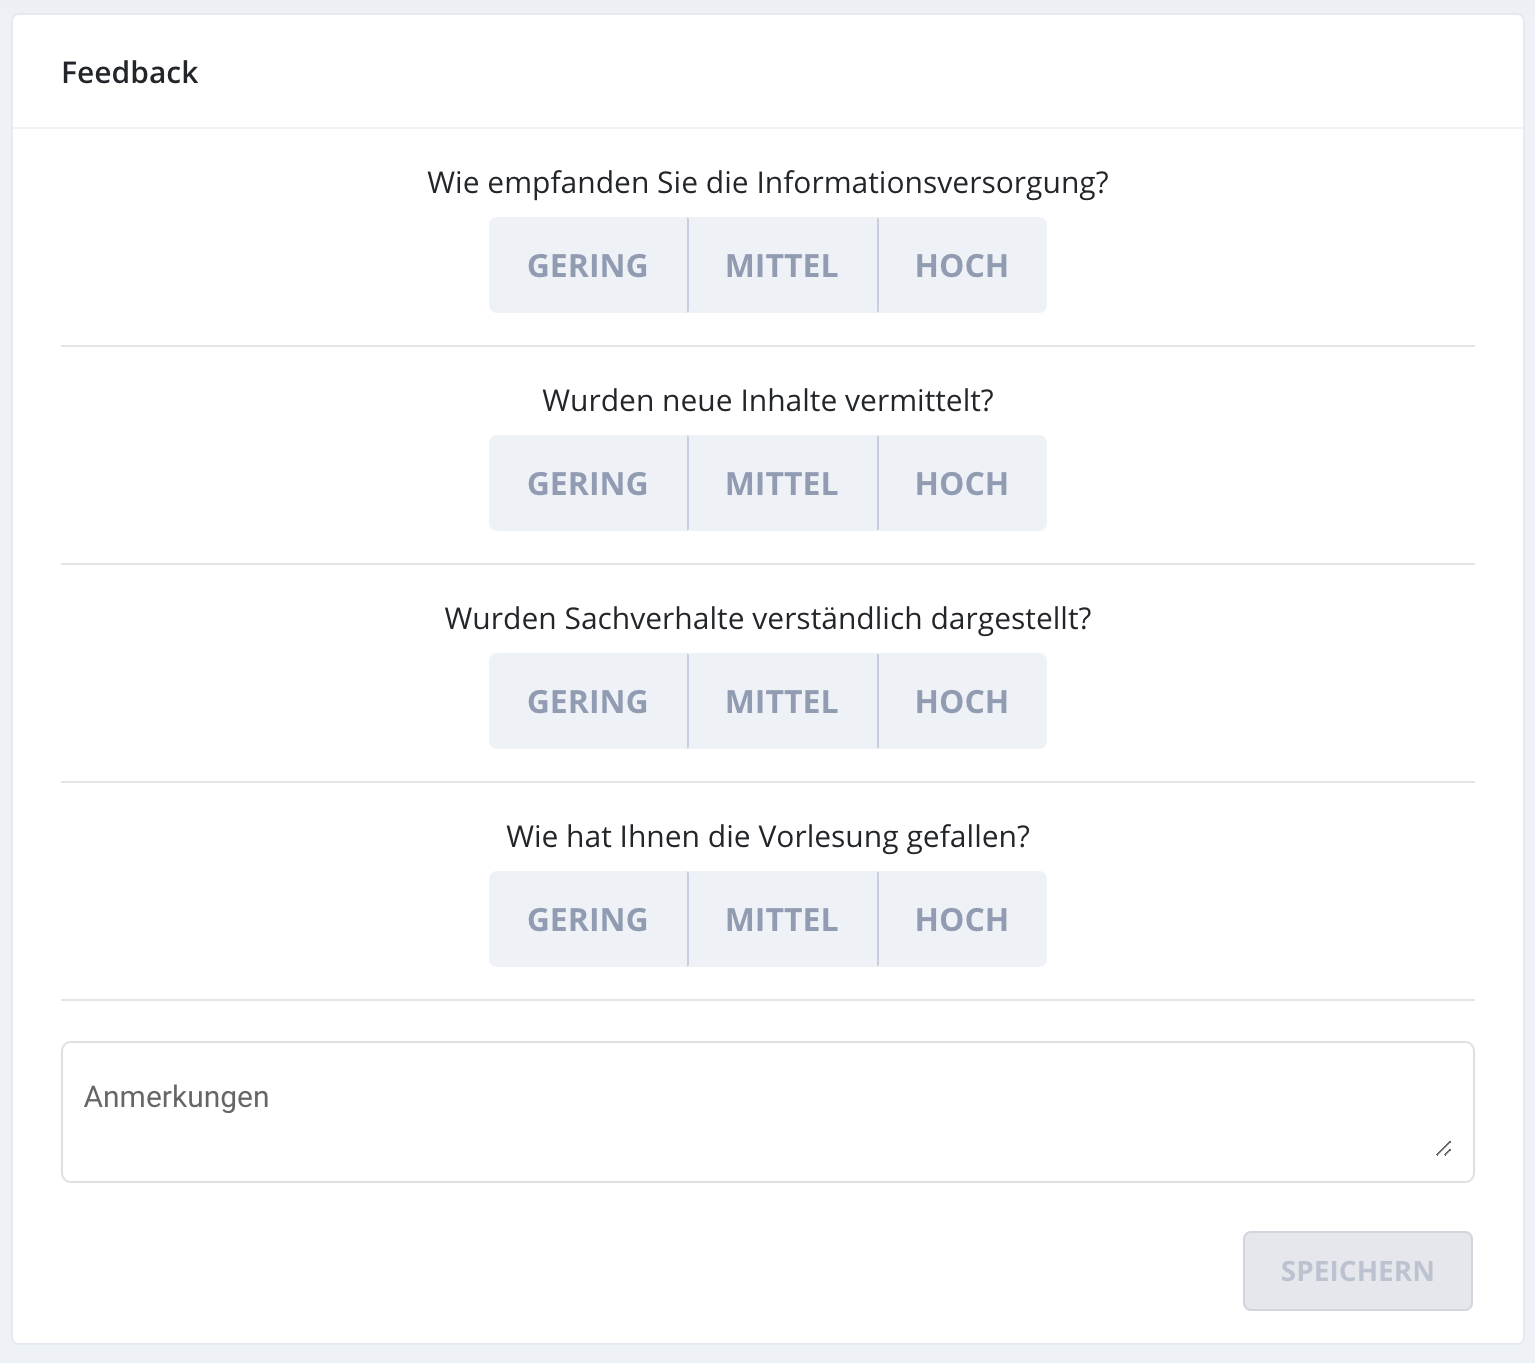
\includegraphics[width=.7\textwidth]{img/Feedback_geben.png}
    \caption{Feedback}
    \label{fig:feedback}
\end{figure}
Der Dozent kann nachdem die Teilnehmer ihr Feedback gegeben haben, die Anworten auswerten. Zum einen kann dies direkt in der Webapplikation ausgewertet werden 
und zum anderen können die Ergebnisse als CSV-Datei exportiert werden und selbstständig ausgewertet werden. In der Abbildung \autoref{fig:feedback_ergebnis} 
wird eine beispielhafte Auswertung angezeigt.
\begin{figure}[!h] 
    \centering
    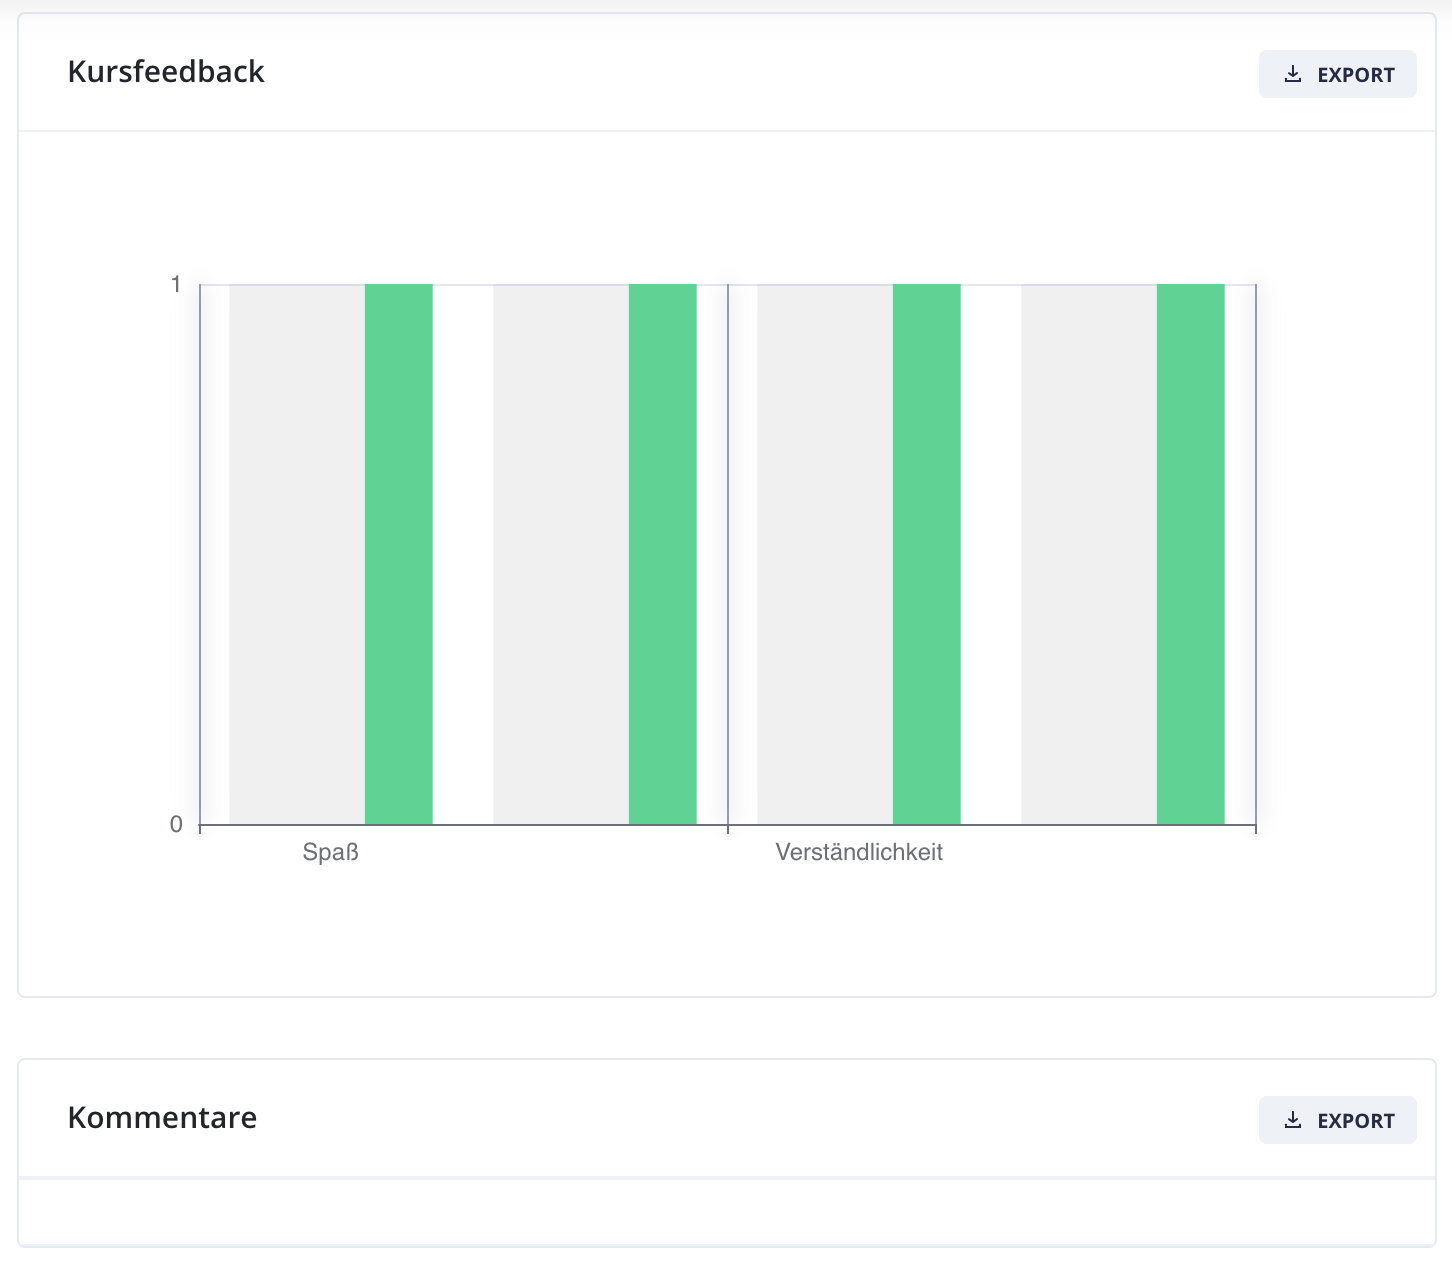
\includegraphics[width=.7\textwidth]{img/Feedback_uebersicht_Teilnehmer_Feedback.png}
    \caption{Feedback-Ergebnis}
    \label{fig:feedback_ergebnis}
\end{figure}
Als letztes Feature bei der Feedbackoption kann eine Übersicht zum Kurs angezeigt werden. Diese Übersicht beinhaltet alle Antworten zu den Fragen, die 
bei der Registrierung gestellt werden. Dadurch hat der Dozent einen Eindruck, welche Arten von Lerntypen in diesem Kurs vertreten sind und wie viel 
Erfahrung die Teilnehmner mit der Online-Lehre haben. 
\begin{figure}[!h] 
    \centering
    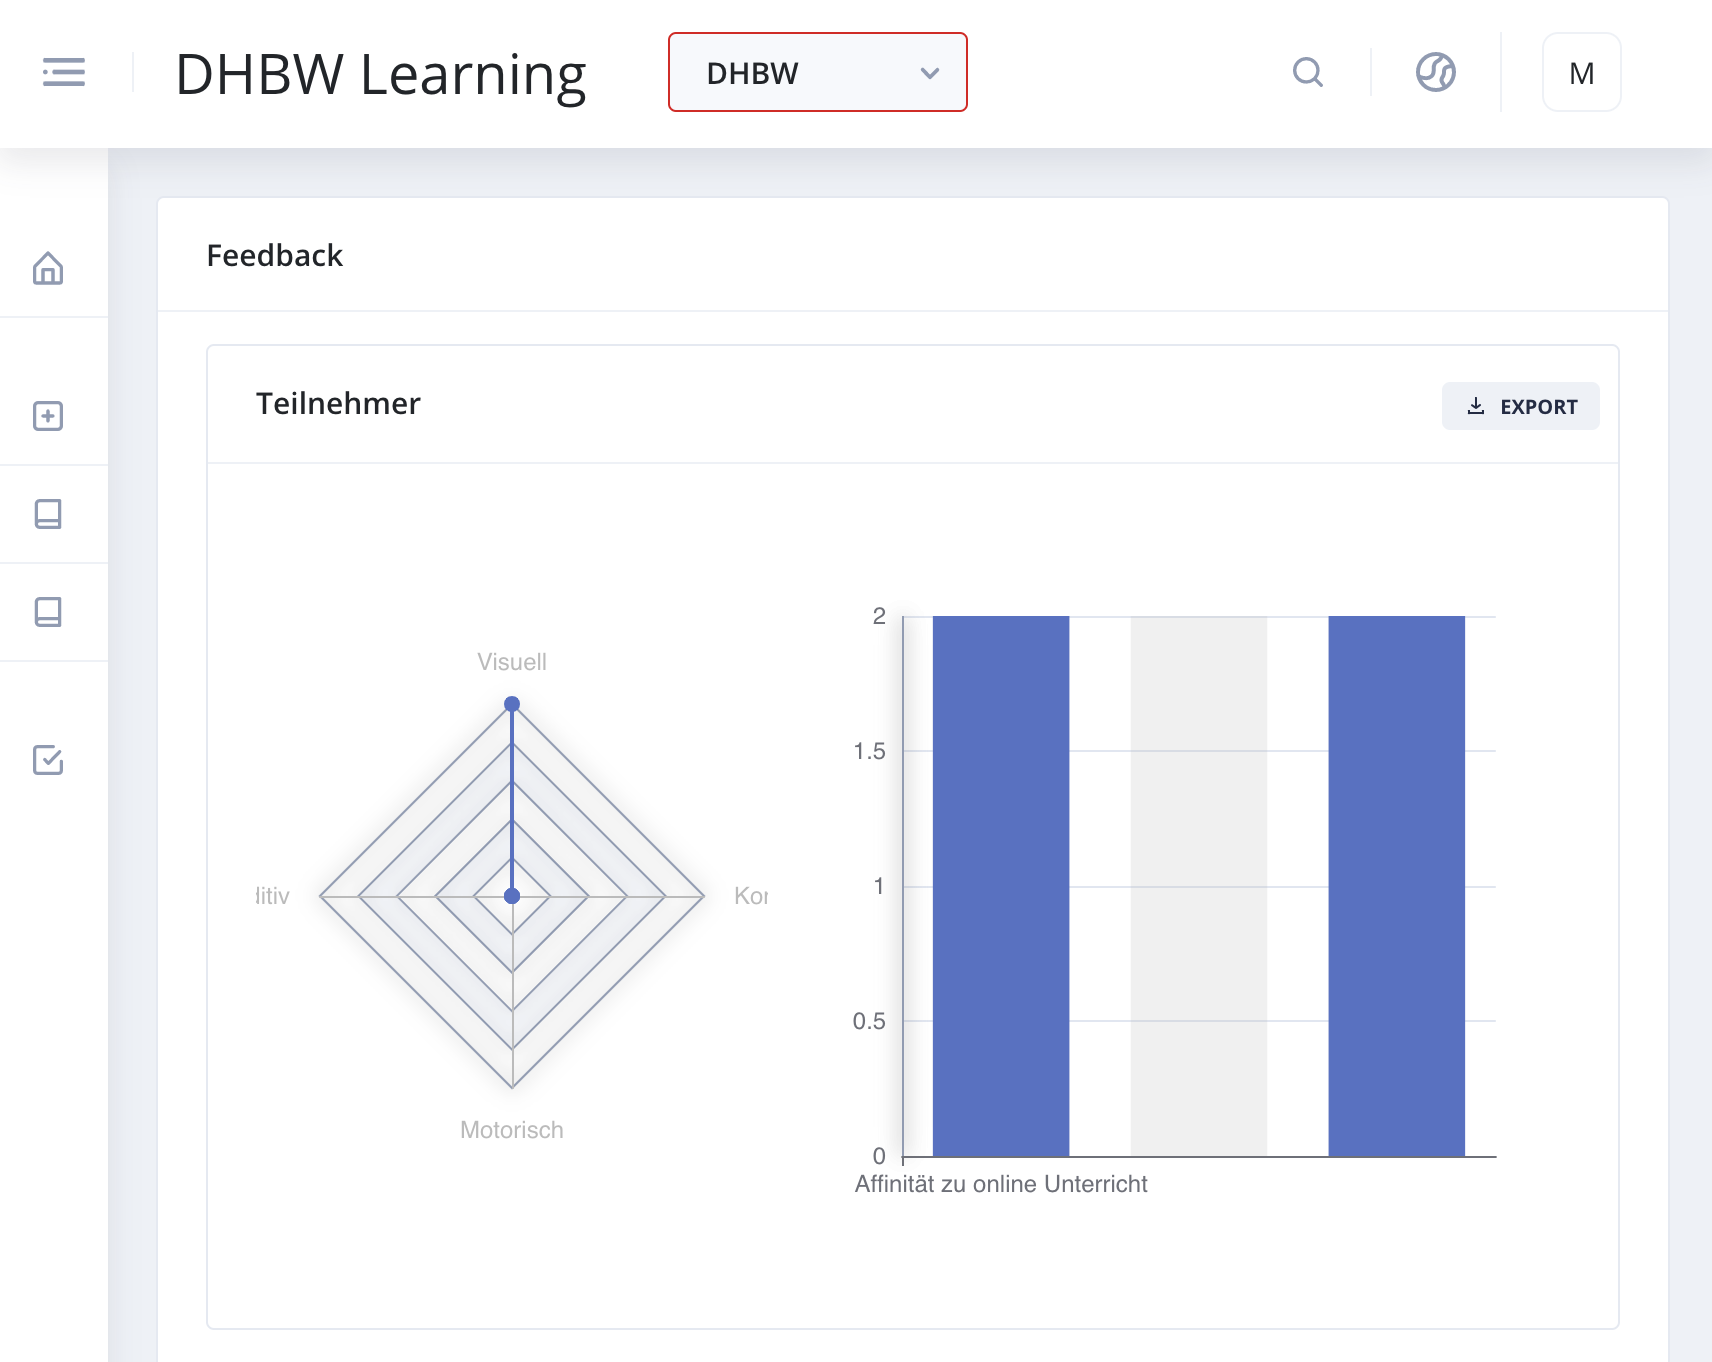
\includegraphics[width=.7\textwidth]{img/Feedback_uebersicht_Teilnehmer.png}
    \caption{Übersicht-Teilnehmner}
    \label{fig:uebersichtTeilnehmner}
\end{figure}




% TODO: Sollte Feedback pro gehaltene Vorlesung sein? -> Einzelne Bereiche einer Vorlesung vertiefen
% Hier kann man vielleicht auch was aus BI sagen, mit Identifikationsfragen, ...
% Lange Umfragen sind blöd



% TODO: Aspekte Learning Analytics
% Das steht schon im Referenzdokument.
% Dann kamm man sagen, Learning Awareness, Privacy Awarness ...  konzentieren wir uns drauf

% TODO: Quotas erwähnen?



\section{Exams}
Als Studenten konnten wir ein weiteres Problem mit der aktuellen Informationsversorgung identifizieren.
Momentan herrscht eine große Unklarheit über Prüfungsleistungen.
Teilweise werden die Prüfungsleistungen in den Vorlesungen angekündigt, manche in Moodle und wieder andere werden in einem Google Calendar eingetragen.
Außer einem Datum sind oft keine weiteren Informationen festgesetzt.
Stattdessen werden diese mündlich in den Vorlesungen bekanntegegeben.
Besonders für Studenten die Aufgrund von Krankheiten oder, in der Zeit von Online-Vorlesungen, Internetverbindugnsprobleme besitzen ist dies problematisch, wenn sie diese Informationen nicht mitbekommen.

Dazu kommt, dass besonders bei Portfolioprüfungen, Prüfungen nicht aus einer einzelnen, sondern aus mehreren Leistungen bestehen.
Ein Beispiel ist die Erstellung einer Präsentation, bei die nicht nur der Vortrag, sondern auch das Begleitmaterial bewertet wird.

Aus diesem Grund können in der Anwendungen Informationen über Klausuren verwaltet werden.
Jede Prüfungsleistung besitzt einen Titel und einer Beschreibung, in der beschrieben werden kann, was die Aufgabe ist.
Außerdem wird das Abgabedatum in einem Kalender zur einfacheren Übersicht dargestellt.
Zusätzlich werden alle wichtigen Informationen, wie Räume oder zugelassenen Hilfsmittel dargestellt.
Die Eingabemaske ist in der Abbildung \autoref{fig:pruefungsmaske} zu sehen.
\begin{figure}[h] 
    \centering
    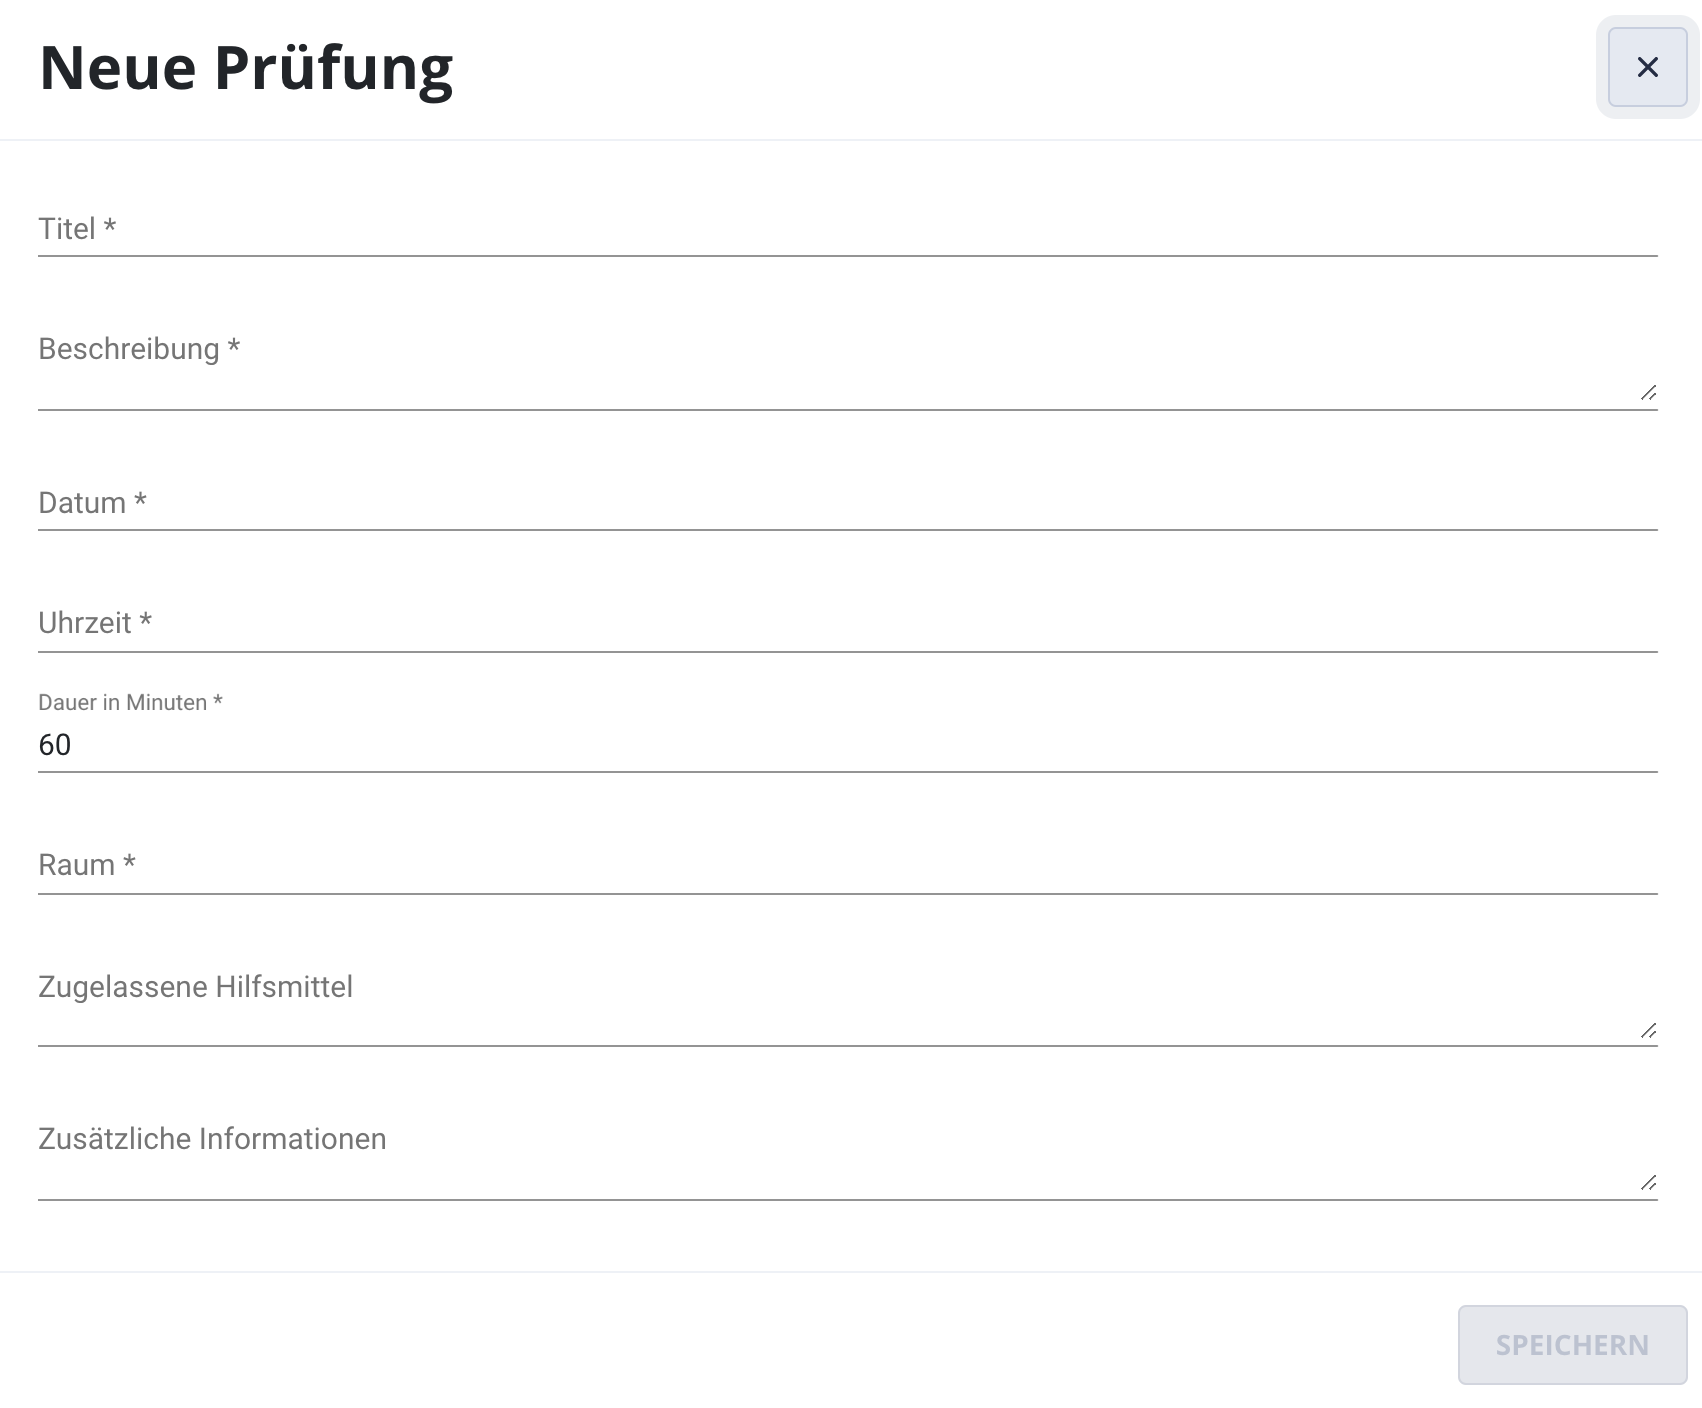
\includegraphics[width=.7\textwidth]{img/Pruefung_hinzugefuegen.png}
    \caption{Prüfungsmaske}
    \label{fig:pruefungsmaske}
\end{figure}
